This section presents \toolname, a \textit{java-based} tool aimed at helping further developers during the testing process of their Android mobile applications. \\
For giving a cleaner and more understandable explanation of how \toolname\ works, I would like to split its key features into three main categories (which should also be executed in a sequential way, in order to exploit the whole \toolname's potentiality): 
\begin{enumerate}
\item the \textsc{Testing} part is in charge of testing a given set of \textit{APKs}, reporting their testing results and extracting possible \textit{crashes} from the before generated test logs; 

\item the \textsc{Clustering} part investigates the similarity between the previous extracted crash logs, using different metrics and strategies, in order to collect they together and create a crash log \textit{bucket}; 

\item the \textsc{Linking} part represents the core feature of \toolname. It pre-processes a set of given \textit{user reviews} as well as the set of the previously created crash logs, in order to prepare and "clean" them for the linking procedure.  Afterwards, it investigates whether it exists a correlation between the stack traces and the user feedbacks, with the aim to link, whether possible, the reviews with the crash logs. 
\end{enumerate}

\section{Testing}
%----------------- FDROID CRAWLER --------------
First of all, if no set of \textit{APKs} is available yet, \toolname\ can be exploited for downloading the needed mobile applications from the \textit{F-Droid API\footnote{LINK API}}. In this direction, as shown in the picture \ref{testing}, the component \FDroidCrawler, is first in charge of  parsing a static structured file (\textit{e.g.} a \textit{csv}-file format), which contains a set of android packages names. 
The path of this file is given in the \textsc{configuration manager}, which contains a set of static properties that get elaborated by \toolname. Second, \textsc{fdroid crawler} searches and then extracts a set of \textit{HTTP links} for those android packages that have been found on the API. Afterwards, it builds the correct \textit{HTTP requests} and finally starts the downloading process, saving the returned \textit{APKs} in a given directory.

%-------------- CONFIGURATION ENVIRONMENT--------------
The first step of the testing part was to build a set of \textit{APKs}, with which to perform the testing process. As said, this can be achieved using either \textsc{fdroid crawler} or can also be manually created. Now, the second step is to prepare and configure the testing environment. 
All the parameters needed for starting a testing session have to be specified in the \textsc{configuration manager}. Figure \ref{config}, shows an example of a simplified set of parameters which must be given a priori in order to launch a testing session. \newpage
\label{config}
\begin{lstlisting}[caption=Properties which get elaborated during the testing sessions]
/**
 * Testing session specifications
 */
MINUTES_PER_APP = 30
NR_OF_ITERATIONS = 5
 
/**
* Test logs directories
*/
MONKEY_DIR = Reports/MonkeyReports
SAPIENZ_DIR = Reports/SapienzReports

/**
 * Monkey parameters
 */
LOG_VERBOSITY = -v 
PACKAGE_ALLOWED = -p
NR_INJECTED_EVENTS = 5000
DELAY_BETWEEN_EVENTS = 10
PERCENTAGE_TOUCH_EVENTS = 15
PERCENTAGE_SYSTEM_EVENTS = 15
PERCENTAGE_MOTION_EVENTS = 15
IGNORE_CRASH = True

/**
* Sapienz parameters
*/
SEQUENCE_LENGTH_MIN = 20
SEQUENCE_LENGTH_MAX = 500
SUITE_SIZE = 5
POPULATION_SIZE = 50
OFFSPRING_SIZE = 50
GENERATION = 100
CXPB = 0.7
MUTPB = 0.3
\end{lstlisting}
The figure above represents a part of the \textsc{configuration manager}, where all the testing parameters for \monkey and \sapienz are specified. An in-depth explanation about these parameters concering \monkey and \sapienz can be found on \cite{monkey}, respectively on \cite{sapienz}.\\
In addition to them, the directories on which the generated test logs are going to be stored must be given as well as the specifications about the testing session. The properties about the testing session consist of two values: 
\begin{itemize}
\item \textsc{minutes\_per\_app}, specifies how many minutes an app will be tested. After that time frame, a time-out occurs and the testing process gets restarted with the next app. 
\item \textsc{nr\_of\_iterations}, specifies how many times the whole dataset will be tested.
\end{itemize}

According to the example \ref{config} above and assuming that the \textit{APKs} set consists in 10 apps, the total estimated testing time for an entire testing session would be: 
\begin{center}
30 min p/a * 10 apps * 5 iterations = 1500 min. (25 hours). 
\end{center}
Once the environment testing variables have been configured, the automated tool with whom the testing is going to be performed must be made explicit. Indeed, it has to be specified as parameter in \textsc{main} \textit{args} (as mentioned before in the section \ref{sec:choicetool}, the tools which can be selected are either \monkey or \sapienz). \\
The last configuration step is to define on which kind of device (\textit{i.e}, a real device, such as a \textit{tablet} or a virtual device, such as an \textit{emulator}) the testing is going to be performed. In addition to them, an additional argument that starts a timer for a better overview during the testing process can also be passed as main argument. \toolname\ supports different types of emulators or real devices running on different android API levels. However, in order to correctly execute \sapienz, the API level shall be the \textit{Android 4.4, KitKat}. \\
The listing below shows an example of a combination of possible parameters that could be given as main arguments. 


\begin{lstlisting}[caption=\toolname\ command line, language=bash]
$ java -\toolname.jar -device -monkey -timer
\end{lstlisting}

%-----------LAUNCH A TESTING SESSION -----------
Once the configuration phase is terminated, \toolname\ is able to start the testing process. 
As shown in the picture \ref{testing}, it manages the component \SessionLauncher, which is in charge of translating the previously specified testing properties into "java readable code" and initializing the testing session. 
Concretely, after \toolname\ invokes \SessionLauncher\ all the attached devices respectively the chosen emulators get initialized, \ie they get rebooted and restarted as root, so that some important write-read-permissions are enabled during the testing session. 
Whether the timer has been given as main argument, it gets also started. \\
Once the initialization step has been completed, \SessionLauncher\  invokes the \AppTester\ component which finally starts the testing session. The Listing~\ref{lst:startsession} gives a simplified code snippet about the beginning of the testing process. 

\begin{lstlisting}[caption=\SessionLauncher\ Code snippet for starting a testing session, ,label={lst:startsession}]
private appTester; 
public void startTestingSession() throws Exception {
        final int NUMBER_ITERATIONS = ConfigurationManager.getNumberOfIterations();
        if (IS_EMULATOR) {
        	   SessionLauncher.initialiseEmulator();
        }
        else {
       	   SessionLauncher.initialiseDevices();
        }
       
        if (isTimer) {
            SessionLauncher.initializeTimer();
        }
        for (int i = 0; i < NUMBER_ITERATIONS; i++) {
            System.out.println("Iteration number " + (i+1));
            this.appTester = new AppTester();
            this.appTester.testAllApp();
        }
}
\end{lstlisting}
First of all, the total number of iterations specified in the \Config\ is read and stored into a constant of type int. After that, all the attached devices (or the chosen emulators) gets statically initialized. According to the boolean variable \textit{isTimer}, a timer may also be started.
Afterwards, a for-loop starts where at each iteration the method \textit{testAllApp()} gets invoked. 
The idea behind this, is that at each iteration a new object of type \AppTester\ is created, so that each created object represents one testing loop of the dataset. 
For this reason, as shown in the figure~\ref{testing}, the \SessionLauncher\ would be able to instantiate infinite times the class \AppTester. However, it must create at least one object of that type in order to start a testing session. 

\AppTester\ and \Cmd\ represent the core components of the whole testing process. Indeed, \AppTester\ can be viewed as brain of the process, since it tells step-by-step to the body, \ie the \Cmd\ component, which commands it has to execute and at what stage of the process it has to perform it. \\
Listing~\ref{lst:apptester} shows a very simplified code snippet of the relation between the two above mentioned components. 
\begin{lstlisting}[caption=Testing mechanism between \AppTester\ and \Cmd\, ,label={lst:apptester}]
/**
* @class: AppTester
*/
public void testAllApp() {
        for (File apk : this.apksDirectory) {
            if (apk.getName().endsWith(".apk") && !apk.isDirectory()) {
                    uninstallApp(apk.getName());
                    installApp(apk.getName());
                    if (IS_MONKEY) {
                        testAppWithMonkey(config.getMonkeyRepDir(), apk.getName());
                    } else if (IS_SAPIENZ) {
                        testAppWithSapienz(config.getSapienzRepDir(), apk.getName());
                    }
            }
        } 
        // waiting to threads to finish 
        File testLog = CmdExecutor.getCurrentLog();
        if (hasCrash(testLog)) {
            generateCrashLog(testLog);
        }
} 
private void testAppWithSapienz(String dest, final String APK_NAME) {
	CmdExecutor.generateReport(dest, CommandLines.SAPIENZ_CMD_LINE(APK_NAME)); 
}

private void testAppWithMonkey(String dest, final String APK_NAME) {
	CmdExecutor.generateReport(dest, CommandLines.MONKEY_CMD_LINE(APK_NAME)); 
}

/**
* @class: CmdExectutor
*/
public static void generateReport(String dest, String cmd){
        Runtime runtime = Runtime.getRuntime();
        Process p = runtime.exec(cmd);
        StreamGobbler output = new StreamGobbler(p.getInputStream(), cmd, dest); 
        output.start();
        writeTestingEndTime(dest);
    }
    
public static File getCurrentLog() {
    return lastGeneratedLog();
}
    
\end{lstlisting}


First of all, \AppTester\ creates a for-loop in which it iterates each \textit{APK} file contained in the \textit{APKs} directory. Once again, this directory is specified in the \Config. 
The first if statement checks whether the file in question has an adequate extension, \ie it is able to be installed on a android mobile device. After that, \AppTester\ uninstalls the concerned \textit{APK}, so that at each iteration of the testing it get reinstalled. This beacause, it may be that an \textit{APK} gets affected by previously generated sequences (\eg a sequence of random events that led the app to an external website). \\
Afterwards, \AppTester\ checks which automated tool has been chosen by the tester, so that it can tell to the \Cmd\ component, which command-line it has to execute. As stated before, \AppTester\ prepares the single testing components such as which \textit{APK}, which tool, which testing parameters, etc., while \Cmd\ executes them without any prior knowledge. \\
After the automated tool has been detected, \Cmd\ is able to concretely start the testing, executing the passed command-line. This is represented in listing \ref{lst:apptester} by the method \textit{generateReport}. Indeed, \Cmd\ uses a single instance of the java-class \textit{Runtime} that allows the application to interact with the environment in which the app is running \cite{runtime}. This is actually achieved by the \textit{Runtime.getRuntime()}. The next line executes with the previously created object the given command-line. Since this method returns a new Process object, the result of the execution is assigned to a separate process. \\
Assigning the execution of each single command-line to a new single separate process brings with it many advantages: 
\begin{itemize}
\item Processes are independent of each other. If the execution of a command-line fails, it can be interrupted without affecting the entire testing process; 
\item Multithreading can be easily supported; Indeed, the component \Stream\ extends the \textit{Thread} java-class which implements the \textit{Runnable} java-interface. Each time a new process comes in, it starts a new thread in this class.
\item Each process has it own timeout. It may be that some command-lines cannot properly terminate and need to be interrupted during their execution.  
\end{itemize}
\Stream, in turn, is in charge of writing the test report. Each time its construct get instantiated in the \textit{generateReport()} method of the \Cmd\ class, it starts a new thread and begins in parallel the writing phase of the log. 
As shown in listing~\ref{lst:gobbler}, the method \textit{run()} overridden from the \textit{Runnable} interface gets automatically per-default invoked when in the \textit{generateReport} method an object of type \textit{StreamGobbler} calls the \textit{start()} method. 
Once the \textit{start()} method is called, the writing phase starts. This phase uses a \textit{PrintWriter} as well as classic \textit{Reader} for writing text on a file.
Before the test log is written, the metadata about the testing environments are appended to the writer. At the end of the process the writer is closed and the thread can terminate. Once the thread is finished, the method \textit{writeTestingEndTime()} in the method \textit{generateReport()} can start. This method complement the metadata writing the testing end time, so that the total testing time can be computed. 





\begin{lstlisting}[caption=\Stream\ code snippet writing a test log, ,label={lst:gobbler}]
/**
* @class: StreamGobbler
*/
@Override
public void run() {
        try {
            Writer writer = new PrintWriter(outputPath, "UTF-8");
            InputStreamReader isr = new InputStreamReader(is);
            BufferedReader br = new BufferedReader(isr);
            String line;
            writer.append(TesterData.getMetaData()); // insert metadata
            while ((line = br.readLine()) != null) {
                System.out.println(" > " + line); // console overview
                writer.append(line).append("\n"); // test log 
            }
            closeWriter();
        } catch (IOException ioe) {
            ioe.printStackTrace();
        }
}
\end{lstlisting}

Listing~\ref{lst:testinglog} shows a short version of a test log of the app \textit{com.danvelazsco.fbwrapper} that has been generated after the execution of \monkey. 

\begin{lstlisting}[caption=Test log of com.danvelazco.fbwrapper, basicstyle=\fontsize{7}{8}\ttfamily,label={lst:testinglog}]
/**
 * Meta-data
 */
Tester Name: Lucas Pelloni
Testing Start Time: 05/04/2017 11:18:29
Testing End Time: 05/04/2017 11:48:30
Total Testing Time: 30 minutes (0.5 hours)
Type of testing: testing on a physical device
Device name: c0808bf731ab321
Percentage of motion events: 2.0% (number of motion events: 60 of 3000 events)
Percentage of system events: 6.0% (number of system events: 180 of 3000 events)
Percentage of touch events: 1.0% (number of touch events: 30 of 3000 events)

/**
 * Test log 
 **/
:Monkey: seed=1495075565065 count=3000
:AllowPackage: com.danvelazco.fbwrapper
:IncludeCategory: android.intent.category.LAUNCHER
:IncludeCategory: android.intent.category.MONKEY
// Event percentages:
//   0: 1.0%
//   1: 2.0%
//   2: 2.4931507%
//   3: 18.698631%
//   4: -0.0%
//   5: 31.164383%
//   6: 18.698631%
//   7: 6.0%
//   8: 2.4931507%
//   9: 1.2465754%
//   10: 16.205479%
:Switch: #Intent;action=android.intent.action.MAIN;category=android.intent.category.LAUNCHER;end
    // Allowing start of Intent { act=android.intent.action.MAIN cat=[android.intent.category.LAUNCHER]
:Sending Trackball (ACTION_MOVE): 0:(4.0,4.0)
:Sending Trackball (ACTION_MOVE): 0:(4.0,-3.0)
:Sending Trackball (ACTION_MOVE): 0:(2.0,-1.0)
:Sending Trackball (ACTION_MOVE): 0:(-5.0,2.0)
:Sending Trackball (ACTION_MOVE): 0:(-5.0,3.0)
    //[calendar_time:2017-05-05 09:48:23.894  system_uptime:717348]
    // Sending event #100
...
\end{lstlisting}

As shown in the figure above, the test logs do not only contain the test results of the tested app, but also the above mentioned meta-data for documenting and retracing the whole testing session.

The testing phase in the "strict sense", \ie the stage where the \textit{APK} gets stressed with an automated tool is over. At this point, the logs must be investigated about the possibility that some apps have generated a crash during its testing time frame. In this sense, the last part of the method \textit{testAllApp()} illustrated in the listing ~\ref{lst:apptester}, is in charge of stating whether a test log contains a crash or not. The method for checking whether a test log has collected a crash inside it is quite intuitive. This because, the syntax used by \monkey and \sapienz in their report for indicating the presence of a crash is the same. As illustrated in the listing~\ref{lst:crashlog}, a crash can be delimited using the following two \textit{Strings}: 
\begin{itemize}
\item Crash beginning: \texttt{"// CRASH: "}
\item Crash end: \texttt{"// "}
\end{itemize}

\begin{lstlisting}[caption=Crash log of com.danvelazco.fbwrapper illustrated within its test log, basicstyle=\fontsize{6}{8}\ttfamily,label={lst:crashlog}]
...
:Sending Trackball (ACTION_MOVE): 0:(3.0,3.0)
:Sending Trackball (ACTION_MOVE): 0:(-4.0,-3.0)
:Sending Trackball (ACTION_MOVE): 0:(3.0,-1.0)
// CRASH: com.danvelazco.fbwrapper (pid 4302)
// Short Msg: java.lang.NullPointerException
// Long Msg: java.lang.NullPointerException
// Build Label: samsung/espressowifixx/espressowifi:4.2.2/JDQ39/P3110XXDMH1:user/release-keys
// Build Changelist: 8291
// Build Time: 1419156873000
// java.lang.NullPointerException
// 	at com.danvelazco.fbwrapper.activity.BaseFacebookWebViewActivity.onKeyDown(BaseFacebookWebViewActivity.java:649)
// 	at com.danvelazco.fbwrapper.FbWrapper.onKeyDown(FbWrapper.java:429)
// 	at android.view.KeyEvent.dispatch(KeyEvent.java:2640)
// 	at android.app.Activity.dispatchKeyEvent(Activity.java:2433)
// 	at com.android.internal.policy.impl.PhoneWindow$DecorView.dispatchKeyEvent(PhoneWindow.java:2021)
// 	at android.view.ViewRootImpl$ViewPostImeInputStage.processKeyEvent(ViewRootImpl.java:3845)
// 	at android.view.ViewRootImpl$ViewPostImeInputStage.onProcess(ViewRootImpl.java:3819)
// 	at android.view.ViewRootImpl$InputStage.deliver(ViewRootImpl.java:3392)
// 	at android.view.ViewRootImpl$InputStage.onDeliverToNext(ViewRootImpl.java:3442)
//     ...
//
:Sending Touch (ACTION_DOWN): 0:(215.0,683.0)
:Sending Touch (ACTION_UP): 0:(163.15541,597.4464)
:Sending Touch (ACTION_DOWN): 0:(243.0,812.0)
...

\end{lstlisting} 
Indeed, the method \textit{generateCrashLog()} (~\ref{lst:generatecrash} in the \textit{testAllApp()} is in charge of extracting the crash(es) from its test log. The parsing technique used by this method is to individuate the beginning of the crash using the \texttt{"START\_CRASH"}  string. Once the start has been individuated, the loop continues to add lines of the log	until it finds the \texttt{"END\_CRASH"} string. Once the end has been reached the loop terminates and \Cmd\ writes the results into an external file, in order to extract the crash. 

\begin{lstlisting}[caption=\AppTester's method for extracting a crash log from its test log,label={lst:generatecrash}]
/**
* @class: AppTester
*/
public void generateCrashLog(File testLog) {
        ...
        ArrayList<String> crashLog = new ArrayList<>();
        Pattern start = Pattern.compile(START_CRASH);
        String line;
        while ((line = in.readLine()) != null) {
            Matcher matcher = start.matcher(line);
            if (matcher.find()) {  // crash start
                while (!line.contains(END_CRASH)) { // crash end
                    crashLog.add(line);
                    line = in.readLine();
                }
            }
        }
        CmdExecutor.writeToFile(crashLog, dest);
    }
\end{lstlisting} 


At this point, the \textit{APK} has been tested, reported, its test logs have been investigated and possible crashes have been extracted. Figure~\ref{fig: apkprocess} summarizes the four components which characterizes the testing process of one application. 
\begin{figure}[htb]
\centering 
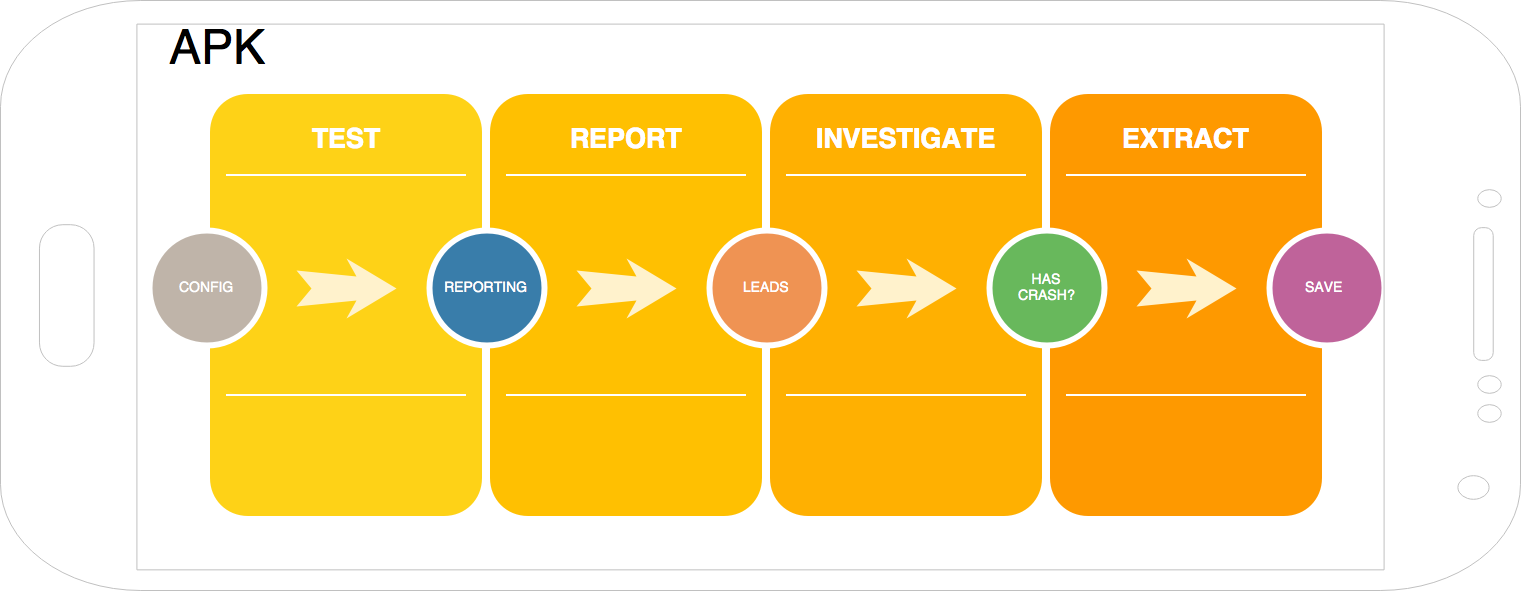
\includegraphics[width=\columnwidth]{imgs/apkprocess} 
\caption{Four test steps performed by \toolname\ of an application}
\label{fig: apkprocess}
\end{figure}



Now, \toolname\ is able to start testing the next application (\ie the next iteration of the loop inside the method \textit{testAllApp())}. 
Once all the applications specified in the dataset have been tested exactly one time, \SessionLauncher\ can begin with the next iteration of its loop (listing ~\ref{lst:startsession}) and so start testing the whole dataset another time. 
This loop ends when the number of iterations reaches the one specified by the user. \\
In addition, during each test iteration and at the end of the whole testing session useful statistics are computed and written into external excel files, using the components \textsc{OnGoingCalculator} and \textsc{FinalCalculator}. They use the pure Java library \textit{Apache POI}, for reading and writing files in Microsoft Office formats \cite{apachepoi}. 




\section{Clustering}
%--------------CLUSTERING AIM-------------
Once the testing phase is finished, all the generated crash logs are stored in a given directory. After this phase, the only way to differentiate them inside this directory is the name of the package for which these crashes occurred. However, among these crash logs there may be a lot of redundancy, since more of them may refer to the same bug. The aim behind the Clustering phase is to create a bucket of unique crash logs. This means, that each crash log has to be compared with the others	 of the same package and according to some metrics that will be explained below, they must be smartly group together. Figure~\ref{fig: clustering} shows the idea behind the Clustering process. 
\begin{figure}[htb]
\centering 
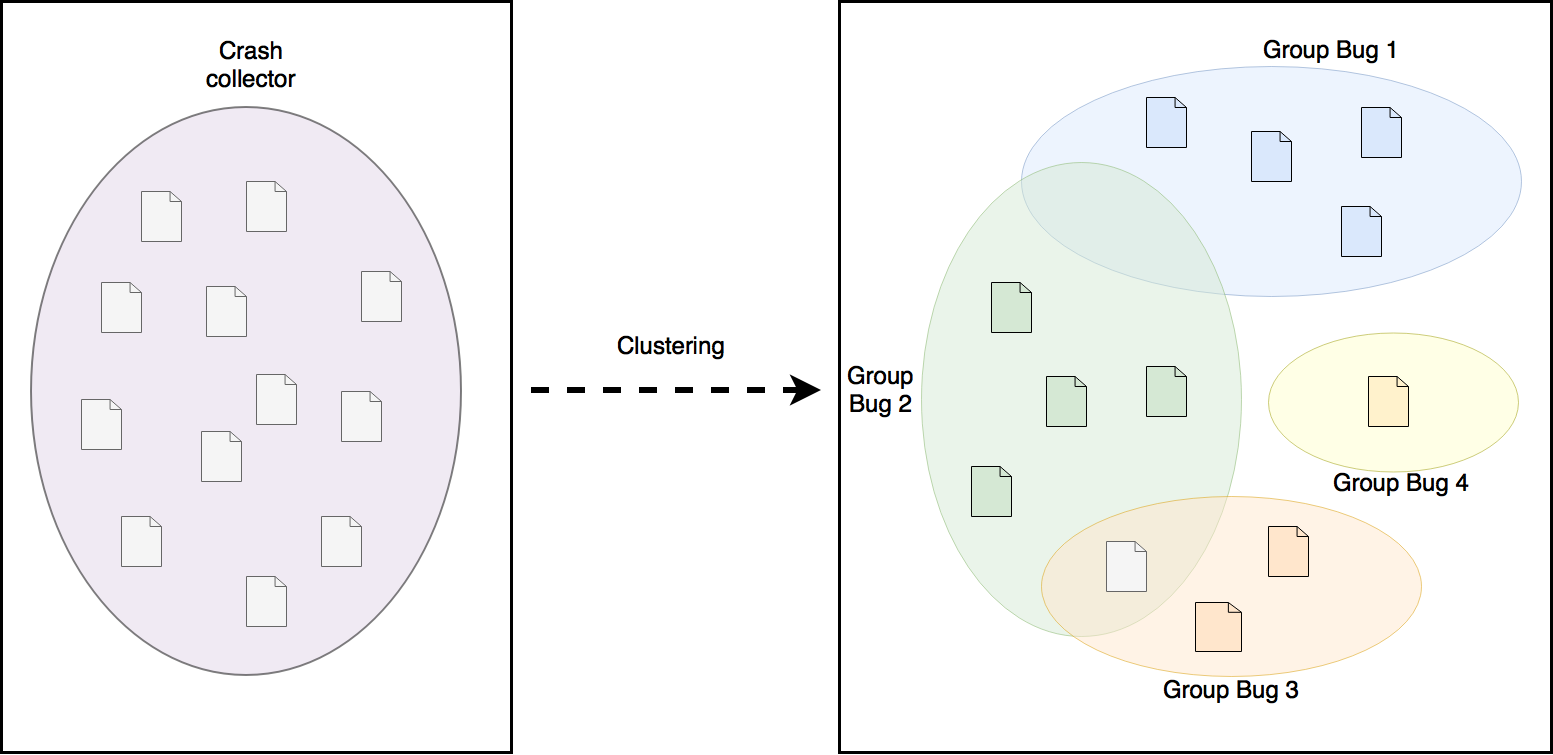
\includegraphics[width=\columnwidth]{imgs/clusteringidea} 
\caption{The idea behind the Clustering process}
\label{fig: clustering}
\end{figure}

Some groups of crash logs may be overlapping. Despite the trigger method, \ie the method that raised to the exception, may be the same, there may be different sequences of function calls in the stack trace, the more the analysis goes deep. However, they are hardly detectable and is difficult to affirm that two stack traces which have the same trigger method refer to different bugs. 

In order to understand better the Clustering approach, a clarification of how a crash log is structured must be done. In order to do this, another example of a crash log is given in the listing~\ref{lst: ringdroid}. 
\begin{lstlisting}[caption=Structure of a crash log, basicstyle=\fontsize{6}{8}\ttfamily,label={lst: ringdroid}]
1.		// CRASH: com.ringdroid (pid 6207)
2.		// Short Msg: android.database.StaleDataException
3.		// Long Msg: android.database.StaleDataException: Attempted to access a cursor after it has been closed.
4.		// android.database.StaleDataException: Attempted to access a cursor after it has been closed.
5.		// 	at android.database.BulkCursorToCursorAdaptor.throwIfCursorIsClosed(BulkCursorToCursorAdaptor.java:64)
6. 		// 	at android.database.BulkCursorToCursorAdaptor.getCount(BulkCursorToCursorAdaptor.java:70)
7.		...
\end{lstlisting}
A crash log is usually structured as follows: 
\begin{itemize}
\item \textit{Line 1} represents the top of the crash log, where the concerned package name is made explicit;
\item \textit{Line 2} tells in few words the cause of the exception; 
\item \textit{Line 3} complements the cause of the exception giving a long explanation about the exception itself;
\item \textit{Line 4} represents the first line of the stack trace. From this point, all the function calls underlying are part of the stack trace;
\item \textit{Line 5} is considered the exact reason for the exception, \ie the trigger method that caused the crash;
\item From \textit{line 6} moving gradually down until the end of the stack trace, there are other nested function calls which contain additional information about the cause of the exception. Usually, the most important ones for identifying the cause are in the first few lines. 
\end{itemize}
Before the explanation of the Clustering process can start, a premise must be made. All the classes that will be discussed below, refer to the class diagram represented in the figure~\ref{clustering}. 


%TODO aggiungere construttore in crash log passandogli gli argomenti
First of all, \toolname\ individuates the directory in which all the previously generated crash logs have been stored. This directory is indicated again in the \Config.\\  
As shown in the listing~\ref{lst: extractor}, \toolname\ loops all the crashes contained inside it and for each of them it calls the method \textit{extractCrashLog()}, in the \Extractor\ component. 

\begin{lstlisting}[caption=\Extractor\ code snippet converting crash files into CrashLog objects,label={lst: extractor}]
/**
* @class: Main
*/
CrashLogExtractor extractor = new CrashLogExtractor();
final String CRASH_CONTAINER = ConfigurationManager.getCrashContainerDirectory();
File[] crash_container = new File(CRASH_CONTAINER).listFiles();
for (File crash : crash_container) {
	extractor.extractCrashLog(crash);
}
\end{lstlisting} 
The method \textit{extractCrashLog()} converts simple crash log files stored inside a folder into \Crash\ Java-objects. 
Indeed, for each crash log file found inside the directory, the constructor of the \Crash\ class get instantiated and so a new object of this type gets created. Each time the constructor of the \Crash\ class gets invoked, it automatically creates the structure of the \Crash-object analogously to the structure of the real crash log file. \\
For instance, the crash log described in the listing \ref{lst: ringdroid} is converted into the \Crash-object represented in the listing~\ref{lst: crashobject}.
It is printed out using the trivial Java method \textit{toString()}, which  per default gives a string representation of the object in question.  

\begin{lstlisting}[caption=\Crash-object,basicstyle=\fontsize{6}{8}\ttfamily, label={lst: crashobject}]
Crash {
	crash_path = /Users/Lucas/Desktop/UZH/BA/CrashLogCollector/crash_log_com.ringdroid.txt
	packageName = com.ringdroid
	Short = android.database.StaleDataException
	Long = android.database.StaleDataException: Attempted to access a cursor after it has been closed.
	first_java_trace_line = android.database.StaleDataException: Attempted to access a cursor after it has been closed.
	trigger_method = [android.database.BulkCursorToCursorAdaptor.getCount(BulkCursorToCursorAdaptor.java:70)]
	trigger_class = BulkCursorToCursorAdaptor
	log_lines = [// CRASH: com.ringdroid (pid 20442), // Short Msg: android.database.StaleDataException, ...]
	
}
\end{lstlisting}
%	all_stack_trace_methods = [BulkCursorToCursorAdaptor, CursorWrapper, MergeCursor,
	 						  %CursorAdapter, AdapterView, AbsListView, ViewGroup, Handler, Looper, ActivityThread, 
	 						  %Method, ZygoteInit]
%augmented_stack_traces = [android, database, stale, attempted, access, cursor, closed, bulk, adaptor, count, wrapper , merge, widget, adapter]  
As you can see in the listing above, the \Crash-object has assumed the same structure as the crash log file. Indeed, it analogously describes the \textit{package name} to which the crash belongs, the \textit{short} and the \textit{long} explanations about the exception, the \textit{trigger method}, etc.
In addition to them, the \Crash-object stores a list of strings containing the log words, where each position of the array is occupied by a different line. 
%-----------LUCENE------------
\paragraph{Preprocessing.}
The second step of the clustering process is to \textit{preprocess} the crash reports in order to prepare them to be compared to each other. 
To achieve this, all the words contained in the crash reports are preprocessed using \textbf{Apache Lucene} \cite{lucene} well-known tokenization techniques.  
Indeed, the \Crash\ class statically invokes for each line the method \textit{tokenizeLine()} in the \Lucene\ class. Listing~\ref{lst: tokenizeline} shows how it concretely works. 
\begin{lstlisting}[caption=Each line inside the crash report is tokenized using \Lucene,label={lst: tokenizeline}]
/**
* @class: CrashLog
*/
private List<String> logLines;
for (String line : this.logLines) {
	LuceneTokenizer.tokenizeLine(line);
}
\end{lstlisting} 
For the tokenization process, \toolname\ uses a well known grammar-based  Lucene-tokenizer, called \textit{StandardTokenizer}. This tokenizer simply split the word fields into lexical units using punctuation and whitespaces as split points. In addition, it removes unnecessary symbols (\eg \texttt{"//"}).
\toolname\ converts all the strings to lowercase and extends the tokenizer with a further regular expression. This because, it's a worldwide convention that developers use CamelCase notation for writing programming words such as names of classes, names of functions or names of variables.
Since most of the words included in the crash logs are programming language keywords, \toolname\ complements the StandardTokenizer of Lucene, so that CamelCase text fields can be also split at the upper-case letters into separate words. 
\clearpage




Consider the following line in the crash report (listing~\ref{lst: ringdroid}) that is passed as argument to the method \textit{tokenizeLine()}: \vspace{-0.8cm}
\begin{center}
\framebox[1\width]{{\fontsize{6.5}{6}{ \texttt{
//\hspace*{0.6cm}at android.database.BulkCursorToCursorAdaptor.throwIfCursorIsClosed(BulkCursorToCursorAdaptor.java:64)}
}}} \par
\end{center}
The following two boxes show the various tokenization steps that are performed by \toolname.
\begin{enumerate}
\item \textbf{Lucene StandardTokenizer}\\ \vspace{0.3em}
\framebox[1\width]{{\fontsize{6.5}{6}{ \texttt{at}
}}}
\framebox[1\width]{{\fontsize{6.5}{6}{ \texttt{android}
}}}
\framebox[1\width]{{\fontsize{6.5}{6}{ \texttt{database}
}}}
\framebox[1\width]{{\fontsize{6.5}{6}{ \texttt{BulkCursorToCursorAdaptor}
}}}
\framebox[1\width]{{\fontsize{6.5}{6}{ \texttt{throwIfCursorIsClosed}
}}}
\framebox[1\width]{{\fontsize{6.5}{6}{ \texttt{BulkCursorToCursorAdaptor}
}}}
\framebox[1\width]{{\fontsize{6.5}{6}{ \texttt{java}
}}}
\framebox[1\width]{{\fontsize{6.5}{6}{ \texttt{64}
}}}
\item \textbf{\toolname\ CamelCase Tokenizer} \\ \vspace{0.3em}
\framebox[1\width]{{\fontsize{6.5}{6}{ \texttt{at}
}}}
\framebox[1\width]{{\fontsize{6.5}{6}{ \texttt{android}
}}} 
\framebox[\width]{{\fontsize{6.5}{6}{ \texttt{database}
}}}
\framebox[\width]{{\fontsize{6.5}{6}{ \texttt{Bulk}
}}}
\framebox[\width]{{\fontsize{6.5}{6}{ \texttt{Cursor}
}}} 
\framebox[\width]{{\fontsize{6.5}{6}{ \texttt{To}
}}}
\framebox[\width]{{\fontsize{6.5}{6}{ \texttt{Cursor}
}}}
\framebox[\width]{{\fontsize{6.5}{6}{ \texttt{Adaptor}
}}} 
\framebox[\width]{{\fontsize{6.5}{6}{ \texttt{throw}
}}}
\framebox[\width]{{\fontsize{6.5}{6}{ \texttt{If}
}}}
\framebox[\width]{{\fontsize{6.5}{6}{ \texttt{Cursor}
}}} 
\framebox[\width]{{\fontsize{6.5}{6}{ \texttt{Is}
}}}
\framebox[\width]{{\fontsize{6.5}{6}{ \texttt{Closed}
}}}
\framebox[\width]{{\fontsize{6.5}{6}{ \texttt{Bulk}
}}} 
\framebox[\width]{{\fontsize{6.5}{6}{ \texttt{Cursor}
}}}
\framebox[\width]{{\fontsize{6.5}{6}{ \texttt{To}
}}} 
\framebox[\width]{{\fontsize{6.5}{6}{ \texttt{Cursor}
}}} 
\framebox[\width]{{\fontsize{6.5}{6}{ \texttt{Adaptor}
}}} 
\framebox[\width]{{\fontsize{6.5}{6}{ \texttt{java}
}}} 
\framebox[\width]{{\fontsize{6.5}{6}{ \texttt{64}
}}} 



\item \textbf{\toolname\ LowerCase Tokenizer} \\ \vspace{0.3em}
\framebox[1\width]{{\fontsize{6.5}{6}{ \texttt{at}
}}}
\framebox[1\width]{{\fontsize{6.5}{6}{ \texttt{android}
}}} 
\framebox[\width]{{\fontsize{6.5}{6}{ \texttt{database}
}}}
\framebox[\width]{{\fontsize{6.5}{6}{ \texttt{bulk}
}}}
\framebox[\width]{{\fontsize{6.5}{6}{ \texttt{cursor}
}}} 
\framebox[\width]{{\fontsize{6.5}{6}{ \texttt{to}
}}}
\framebox[\width]{{\fontsize{6.5}{6}{ \texttt{cursor}
}}}
\framebox[\width]{{\fontsize{6.5}{6}{ \texttt{adaptor}
}}} 
\framebox[\width]{{\fontsize{6.5}{6}{ \texttt{throw}
}}}
\framebox[\width]{{\fontsize{6.5}{6}{ \texttt{if}
}}}
\framebox[\width]{{\fontsize{6.5}{6}{ \texttt{cursor}
}}} 
\framebox[\width]{{\fontsize{6.5}{6}{ \texttt{is}
}}}
\framebox[\width]{{\fontsize{6.5}{6}{ \texttt{closed}
}}}
\framebox[\width]{{\fontsize{6.5}{6}{ \texttt{bulk}
}}} 
\framebox[\width]{{\fontsize{6.5}{6}{ \texttt{cursor}
}}}
\framebox[\width]{{\fontsize{6.5}{6}{ \texttt{to}
}}} 
\framebox[\width]{{\fontsize{6.5}{6}{ \texttt{cursor}
}}} 
\framebox[\width]{{\fontsize{6.5}{6}{ \texttt{adaptor}
}}} 
\framebox[\width]{{\fontsize{6.5}{6}{ \texttt{java}
}}} 
\framebox[\width]{{\fontsize{6.5}{6}{ \texttt{64}
}}} 
\end{enumerate}
This tokenization process is repeated for all lines of all crash reports stored in the directory. At the end of this process, each \Crash-object is complemented with a new attribute which represents the set of preprocessed words.

\paragraph{TF-IDF.} After the phase of preprocessing, the crash logs are ready to be bucketed. In order to classify them, some well-known bucketing techniques are implemented by \toolname, with the aim to deduplicate the greatest number possible of crash reports.
In this direction, \toolname\ implements a \textit{tf-idf} algorithm \textit{(term frequency–inverse document frequency)}, a well-know term-weighting scheme used in information retrieval or text mining \cite{tfidf}. Indeed, tf–idf is a way to measure the relevance, the weight of a term compared to its document or its entire document collection (in our case, the crash logs). The importance of a term is given by the number of times it occurs in a particular document, inversely proportional to its appearance in the entire documents collection \cite{campbell}.  \\
Generally, a tf-idf algorithm consists in three main components \cite{tfidfsimilarity}: 
\begin{itemize}
\item \textbf{TF (Term Frequency)}, \ie how many times a term appears in the currently scored document, where repeated terms indicate the topic of the document; A high TF means that the word in question has a high relevance for the document. The following simplified equation \cite{tfidf} describes a formula for calculating the term frequency:
\begin{align*}
tf_{x,y} = \frac{n_{x,y}}{\mid d_{y} \mid}
\end{align*}
where $n_{x,y}$ represents the number of occurrences of the term $t_x$ in the document $d_{y}$, while $\mid d_{y} \mid$ represents the number of words inside the document $d_{y}$.

\item \textbf{IDF (Inverse Document Frequency)}, \ie the inverse of the document frequency, that represents the number of document in which the term appears. If the same term appears in fewer documents, IDF shows a high value, if a term is very common it returns a low value. 
The equation \cite{tfidf} below describes a simplified version of the inverse document frequency formula: 
\begin{align*}
idf_{x} = \frac{\mid D \mid}{\mid \{d: t_{i} \in d\} \mid}
\end{align*}
where $\mid D \mid$ is the number of documents in the collection, while $\mid \{d: t_{i} \in d\} \mid$ represents the number of documents which contains the term $t_i$

\item \textbf{TF-IDF}, \ie the product of the two above terms. If it has a high value means that the currently scored term has a high relevance, otherwise if it returns a low value, the term has little relevance.
\begin{align*}
tfidf_{x,y} = tf_{x,y}*idf_{x}
\end{align*}

\end{itemize}
The IDF metric actually measures how important a term is. This because, a term which appears very often in a single document will have a high TF score but if this term rarely occurs in the other ones it will also have have a high IDF score and so a low TF-IDF value. This would imply that it shall not have a high relevance. Otherwise, if a word occurs very often both in a single document and in the entire collection it has a high TF score and a low IDF-value, which results in a high TF-IDF score. \\

\toolname\ implements a \textit{tf-idf} scheme, computing TF-IDF scores for all words within all crash logs using again the \textbf{Apache Lucene} library. \\
First of all, \toolname\ creates an index using an \texttt{IndexWriter}. The following diagram illustrates the main components of the Lucene indexing process:
\begin{figure}[htb]
\centering 
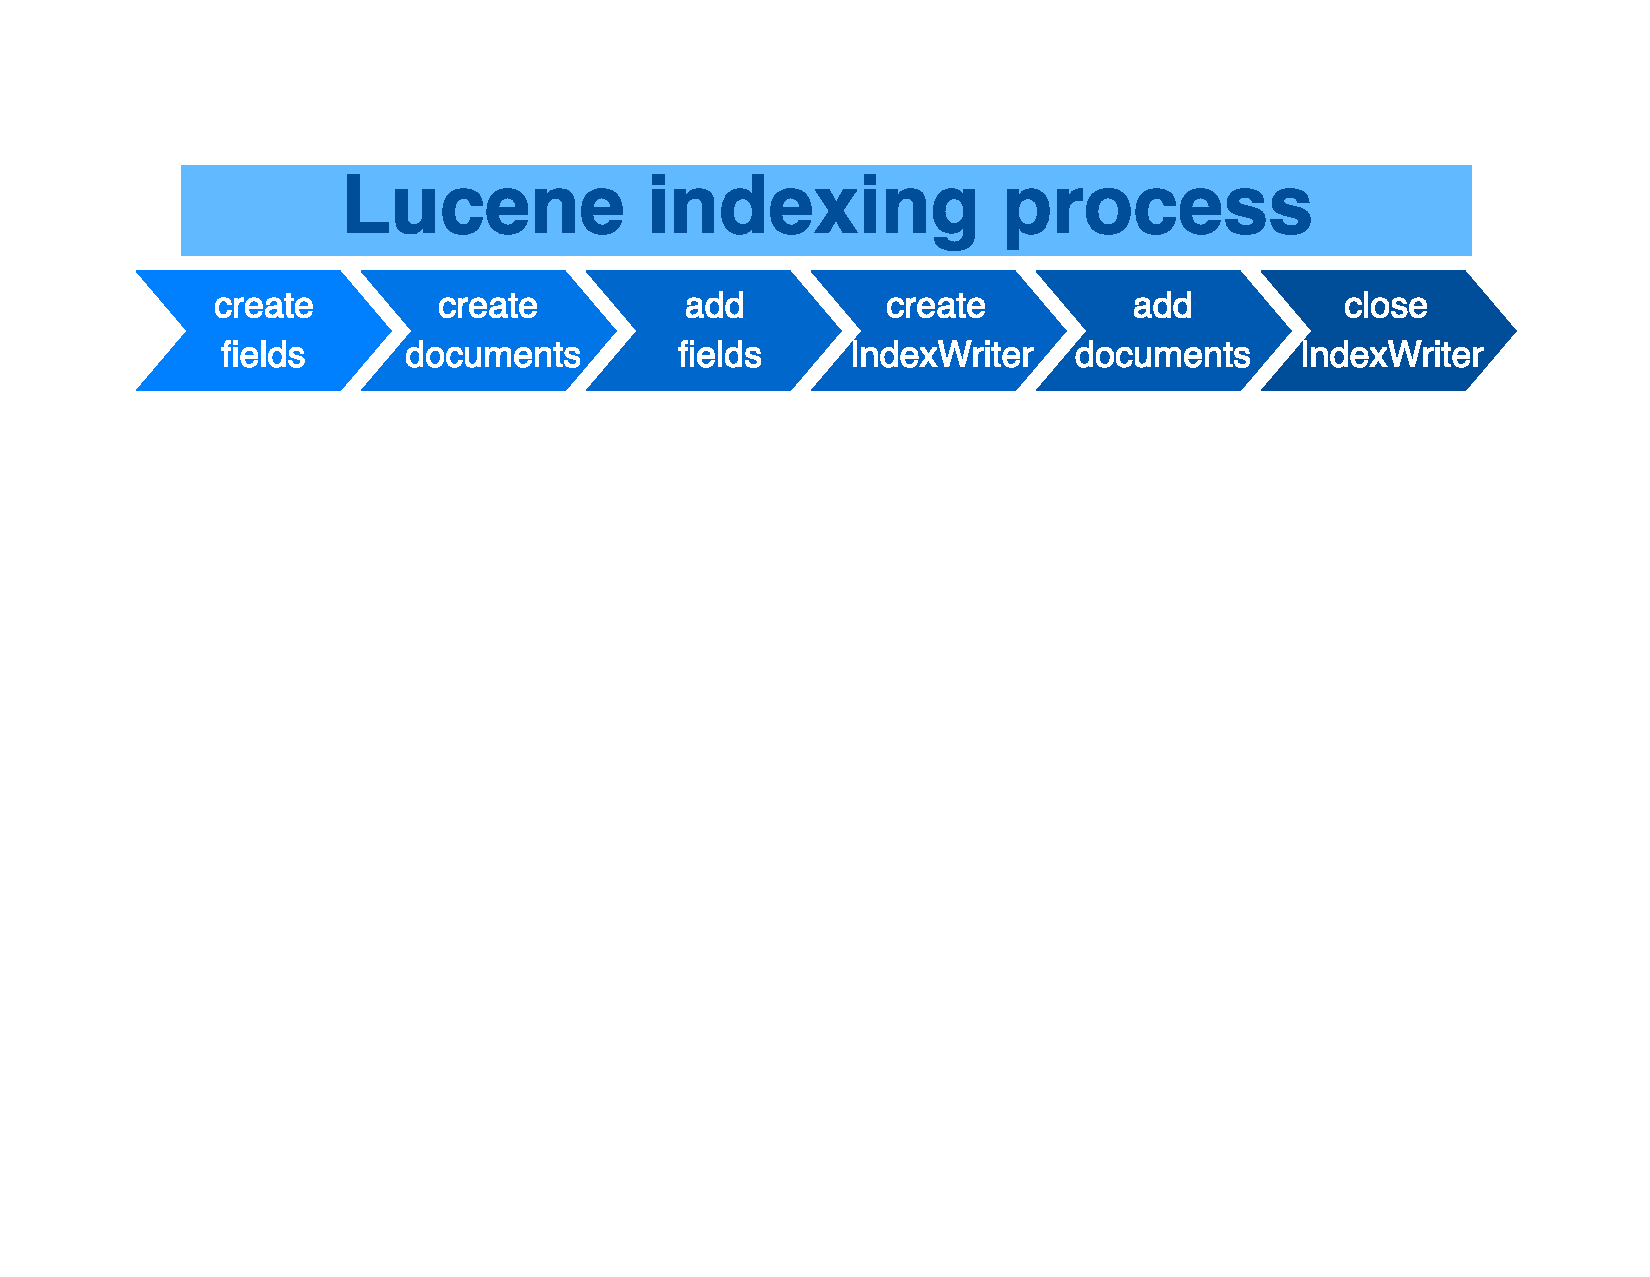
\includegraphics[width=\columnwidth]{diagrams/indexingProcess} 
\caption{Apache Lucene indexing process}
\label{fig: indexingprocess}
\end{figure}

\paragraph{Creating documents and adding fields.}
The first step \toolname\ performs is to create a set of \textit{Lucene documents}. 
To do this, it goes through all previously created \Crash-objects and convert their preprocessed words into Lucene documents. Each document must contain its group of \textit{fields} in order to be indexed.
Therefore, each time a new Lucene document is created, a set of fields must be set and enclosed inside it. 
A field can be viewed as a section of a document which can be optionally stored in the index \cite{lucenefield} and usually has three components: name, type and content. For each stored field, it is important to determine which type is best suited to the content that is going to be indexed. 
For instance, \toolname\ indexes documents which enclose \textit{text fields}, since they are already stored, tokenized and indexed \cite{lucenetextfield}. 
In order to be able to compute TF-IDF values for the indexed Lucene documents, \toolname\ must enable the property that they can have \textit{term vectors}, \ie they can store "a list of the document's terms and their number of occurrences in that document" \cite{lucenetermvector}. \\
The first steps of the Lucene indexing process can be summarized by the following code snippet, which is a simplified version of the \textit{createIndex()} method, illustrated in the diagram~\ref{clustering}.

\begin{lstlisting}[caption=\TFIDF\ describing the Lucene indexing process,label={lst: indexing}]
/**
* @class: TFIDFCalculator
*/
private void createIndex(List<CrashLog> crashLogs) throws IOException {
			// TODO: create IndexWriter
            for (CrashLog crash : crashLogs) {
                ArrayList<String> crash_log_words = crash.getSetOfWords();
                // type of field is set
                FieldType fieldType = new FieldType(TextField.TYPE_STORED); 
                // term vector is enabled
                fieldType.setStoreTermVectors(true); 
                // new document is created
                Document doc = new Document(); 
                for (String word : crash_log_words) {
                    // fields are added into the documents
                    doc.add(new Field(LConstants.FIELD_NAME, word, fieldType)); 
                }
                doc.add(new Field(LConstants.FIELD_ID, crash.getPath(), fieldType));
            }
\end{lstlisting} 
As shown in the listing above, \toolname\ goes through all the given crash logs and stores in a local list their preprocessed log words. 
Afterwards, the field type \textit{TextField} is selected. 
In the next line, the above mentioned term vector property is enabled. Then, a new Lucene document is generated. 
At this point, \toolname\ goes through each preprocessed word and at each iteration adds the current word to a new field which has just been created. The new field has a name, a content, \ie the word in question and a type, \ie the previously selected field type. Finally, the entire field is added to the document. At the end of the loop an additional field is added and used as ID for the document (in our case, the crash log path acts as unique attribute in the index). 

\paragraph{Creating IndexWriter and adding documents.}
In order to index Lucene documents, \toolname\ must generate an \textit{IndexWriter}. This because, this object acts as a core component for creating and updating indexes. 
First of all, \toolname\ creates an object of type \textit{IndexWriter}. However, the instantiating process of this class requires some supplementary configurations that must be passed to the constructor in order to create a new object of that type. 
These two information consist in (i) the directory where the index should point at and (ii) the Lucene \textit{Analyser} which is in charge of analysing the indexed documents. 
After the specification of these two information, a new object of type \textit{IndexWriter} can be created. 
Once created, all documents can be added to the index. At the end of the indexing process the writer must be closed.\\
The listing below complements the code snippet~\ref{lst: indexing} with the instantiation of the \textit{IndexWriter} class and consequentially with the addition of the documents to the index.  
\begin{lstlisting}[caption=\TFIDF\ describing the instantiation of an IndexWriter,label={lst: indexwriter}]
/**
* @class: TFIDFCalculator
*/
private void createIndex (List<CrashLog> crashLogs) throws IOException {
			// directory gets specified
		    FSDirectory dir = FSDirectory.open(new File("\Users\Lucas\Desktop\BA\Index").toPath());
		    // configuration is set
            IndexWriterConfig config = new IndexWriterConfig(new StandardAnalyzer());
            // IndexWriter gets instantiated 
            IndexWriter writer = new IndexWriter(dir, config);
	
            for (CrashLog crash : crashLogs) {
                ArrayList<String> crash_log_words = crash.getSetOfWords();
                FieldType fieldType = new FieldType(TextField.TYPE_STORED); 
                fieldType.setStoreTermVectors(true); 
                Document doc = new Document(); 
                for (String word : crash_log_words) {
                    doc.add(new Field(LConstants.FIELD_NAME, word, fieldType)); 
                }
                doc.add(new Field(LConstants.FIELD_ID, crash.getPath(), fieldType));
                // document are added to the index using an IndexWriter object
                writer.addDocument(doc);
   			}
                writer.close();
}
    
\end{lstlisting} 
As illustrated in the example above, the location where the index should point at can be inserted using the Lucene class \textit{FSDirectory}. It is a base class for Directory implementations that store index files in the file system \cite{lucenefsdir}. Next line of code, the analyser which is used for analysing the Lucene documents is defined. This can made using the Lucene class \textit{IndexWriterConfig}, which holds all the configuration that is used to create an \textit{IndexWriter}. \toolname\ defines again a \textit{StandardAnalyser}, the same used for preprocessing the crash logs.
Finally, a new \textit{IndexWriter} can be constructed per the previously configured settings. 
Once an \textit{IndexWriter} is created, all Lucene documents can be added to the index using a simple method called \textit{addDocument()}. At the end of the indexing process all preprocessed words contained inside the \Crash-objects have been converted into Lucene documents and have been indexed.


\paragraph{Computing TF-IDF scores.} At this point, the index has been created and each document has the possibility to store its vector of terms so that TF-IDF values can be computed for each word of each term of vector of each crash report. 
In this direction, \toolname\ invokes the \textit{computeScoreMap()} method in the \TFIDF\ class, which returns a hash map object. 
This hash map has as keys the unique locations of the crash logs, each one of them is associated with another hash map which contains the term vector.
Table ~\ref{tbl: scoremap} shows the structure of the hash map, taking as a reference the crash log presented in the listing ~\ref{lst: ringdroid}. 
\begin{table}[htb]
\centering
\caption{Structure of the hash map containing its term vector}
\label{tbl: scoremap}
\begin{tabular}{l|c|c|}
\hline
\multicolumn{1}{|c|}{{\color[HTML]{000000} \textit{\textbf{Crash log path (key)}}}}                                 & \multicolumn{2}{c|}{{\color[HTML]{000000} \textit{\textbf{HashMap (value)}}}} \\ \hline
\multicolumn{1}{|l|}{\textit{../Desktop/BA/CrashLogCollector/crash\_log1\_com.ringdroid.txt}} & {\textit{term (key)}}                   & { \textit{tfidf (value)}}                  \\ \hline
                                                                                                            & \hspace{0.7cm}exception\hspace{0.7cm}                             & \hspace{0.2cm}1.73\hspace{0.2cm}                                      \\ \cline{2-3} 
                                                                                                            & view                               & 5.12                                  \\ \cline{2-3} 
                                                                                                            & accessibility                         & 4.77                                  \\ \cline{2-3} 
                                                                                                            & crash                                 & 1.00                                  \\ \cline{2-3} 
                                                                                                            & scrollable                            & 1.92                                  \\ \cline{2-3} 
                                                                                                            & adapter                               & 2.44                                  \\ \cline{2-3} 
                                                                                                            & ringdroid                             & 1.00                                  \\ \cline{2-3} 
                                                                                                            & ...                             & ...                                  
\end{tabular}
\end{table}

As shown in the table above, the terms which have the highest tf-idf relevance are \textit{accessibility} and \textit{view}. Indeed, they have a high term frequency in the currently scored crash log and a low document frequency of the term in the entire collection. 
Terms such as \textit{crash} or \textit{ringdroid} have a low tf-idf weight. In fact, they are generic and irrelevant terms, since they don't give any useful information about the topic of the document. \\
\toolname\ computes tf-idf scores for all vector terms of all crash logs. Once this processed is completed, the similarity between the set of crash logs stored inside the hash map can be computed.
\paragraph{Cosine similarity.} 
In order to state whether two crash logs refer to the same bug, \ie they can belong to the same group in the bucket, \toolname\ computes cosine similarity between the previously generated vectors terms. 
The cosine similarity is just a measure of similarity between two vectors \cite{cosine} (in our case, two normalized weighted vectors consisting of their tf-idf scores).
Usually, the resulting similarity ranges from -1 to 1, but in the case of information retrieval, since the frequency of the terms are always positive, the returned values range from 0 to 1, where 0 indicates that two documents are completely decorrelated, while 1 means that the words contained inside them are exactly the same.  
The equation describing the cosine similarity between two vectors is as follows: 
\begin{align*}
cosine\:similarity = \cos({\theta}) = \frac{A\cdot{B}}{||A||\:||B||}
\end{align*}
where, in our case $A$ and $B$ are two normalized weighted term vectors consisting of tf-idf values. 
With the term "normalized" is understood that when two weighted vectors are used to compute cosine similarity among them, for each time a word is contained within a vector but not in the other, the vector that does not contain the term gets complemented with it by associating a tf-idf score of 0. In doing so furthermore, the two vectors have the same length so that their dot product can be computed.
Figure below shows how the normalization process works. 

\begin{table}[htb]
\centering
\caption{Vector terms $A$ and $B$ before normalization}
\label{tbl: beforenormal}
\begin{tabular}{ccllcc}
\cline{1-2} \cline{5-6}
\multicolumn{2}{|c|}{{\color[HTML]{000000} \textit{\textbf{Vector A}}}}     &  & \multicolumn{1}{l|}{} & \multicolumn{1}{c|}{{\color[HTML]{000000} \textit{\textbf{Vector B}}}} & \multicolumn{1}{c|}{}                \\ \cline{1-2} \cline{5-6} 
\multicolumn{1}{|c|}{\textbf{terms}} & \multicolumn{1}{c|}{\textbf{tf-idf}} &  & \multicolumn{1}{l|}{} & \multicolumn{1}{c|}{\textbf{terms}}                                    & \multicolumn{1}{c|}{\textbf{tf-idf}} \\ \cline{1-2} \cline{5-6} 
\multicolumn{1}{|c|}{handler}        & \multicolumn{1}{c|}{3.15}            &  & \multicolumn{1}{l|}{} & \multicolumn{1}{c|}{exception}                                         & \multicolumn{1}{c|}{1.73}            \\ \cline{1-2} \cline{5-6} 
\multicolumn{1}{|c|}{accessibility}  & \multicolumn{1}{c|}{1.7}             &  & \multicolumn{1}{l|}{} & \multicolumn{1}{c|}{handler}                                           & \multicolumn{1}{c|}{2.01}            \\ \cline{1-2} \cline{5-6} 
\multicolumn{1}{|c|}{crash}          & \multicolumn{1}{c|}{1.13}            &  & \multicolumn{1}{l|}{} & \multicolumn{1}{c|}{accessibility}                                     & \multicolumn{1}{c|}{4.77}            \\ \cline{1-2} \cline{5-6} 
\multicolumn{1}{|c|}{invoke}         & \multicolumn{1}{c|}{1.41}            &  & \multicolumn{1}{l|}{} & \multicolumn{1}{c|}{crash}                                             & \multicolumn{1}{c|}{1.00}            \\ \cline{1-2} \cline{5-6} 
\multicolumn{1}{|c|}{ringdroid}      & \multicolumn{1}{c|}{1.00}            &  & \multicolumn{1}{l|}{} & \multicolumn{1}{c|}{scrollable}                                        & \multicolumn{1}{c|}{1.92}            \\ \cline{1-2} \cline{5-6} 
                                     & \textbf{}                            &  & \multicolumn{1}{l|}{} & \multicolumn{1}{c|}{adapter}                                           & \multicolumn{1}{c|}{2.44}            \\ \cline{5-6} 
                                     &                                      &  & \multicolumn{1}{l|}{} & \multicolumn{1}{c|}{ringdroid}                                         & \multicolumn{1}{c|}{1.00}   \\ \cline{5-6} 
                                     &                                      &  &                       &                                                                        &                                     
\end{tabular}
\end{table}

\begin{table}[htb]
\centering
\caption{Normalized weighted vector terms $A$ and $B$}
\label{tbl: afternormal}
\begin{tabular}{|c|c|c|c|}
\hline
\multicolumn{2}{|c|}{{\color[HTML]{000000} \textit{\textbf{Vector A}}}} & \multicolumn{2}{c|}{{\color[HTML]{000000} \textit{\textbf{Vector B}}}} \\ \hline
\textbf{terms}                     & \textbf{tf-idf}                    & \textbf{terms}                    & \textbf{tf-idf}                    \\ \hline
\textbf{exception}                          & \textbf{0}                         & exception                         & 1.73                               \\ \hline
handler                            & 3.15                               & handler                           & 2.01                               \\ \hline
accessibility                      & 1.7                                & accessibility                     & 4.77                               \\ \hline
crash                              & 1.13                               & crash                             & 1.00                               \\ \hline
\textbf{scrollable}                         & \textbf{0}                         & scrollable                        & 1.92                               \\ \hline
\textbf{adapter}                            & \textbf{0}                         & adapter                           & 2.44                               \\ \hline
invoke                             & 1.41                               & \textbf{invoke}                            & \textbf{0}                         \\ \hline
ringdroid                          & 1.00                               & ringdroid                         & 1.00                               \\ \hline
\end{tabular}
\end{table}
As shown in the tables above, the vectors $A$ and $B$ after the normalization process have the same length and have been complemented with their missing words. 

\paragraph{Computing Cosine Similarity to create the bucket.}
Once the vector terms have been normalized, the cosine similarity among crash reports can be computed. \\
In this direction, \toolname\ defines a threshold in the class \Oracle\,  which represents the tolerance for evaluating the similarity between two crash reports. Indeed, if the calculated cosine similarity among them is greater than the given limit, the two crash logs are considered to describe the same bug, \ie they will belong to the same bug group in the bucket. \\
Concretely, \toolname\ invokes the method \textit{fillCrashLogBucket()}, which is in charge of comparing the crash logs, classifying them with the aim of filling the bucket. 
The bucket consists of a hash map, which has as keys a set of strings which act as a labels for the entire bug group they represent. Each label, in turn, has its own list of \Crash-objects\, which have been considered by the \Oracle\ referring to the same bug.  \\
The bucketing process iterates all crash reports and it concretely works as follows: 
\begin{enumerate}
\item The method \textit{fillCrashLogBucket()} firstly extracts the first crash log in the list and insert it into the bucket, assigning to it the label of the first bug group. 
\item Starting from the second iteration, \toolname\ computes the cosine similarity between the current crash log and all crash logs which are placed at the first position in the list of the other bug groups. 
\item Whether all computed similarities are smaller than the threshold provided by the \Oracle\, means that there is no crash logs in the bucket already which can be considered the same as the current one. For this reason, \toolname\ creates a new bug group with a new label and insert into it the current crash log. \\
Otherwise, in the event that there is at least one computed similarity which is greater than the threshold, \toolname\ extracts the group inside the bucket which shows the highest similarity with the crash log and insert it into it.
In doing so, it gets added into the group which "resemble it more". 
\end{enumerate}
The \textit{BPMN}\footnote{Business Process Model and Notation} diagram \ref{bucketing} explains and summarizes the above mentioned bucketing process provided by \toolname. \\

\begin{figure}[htb]
\centering 
%	\vspace{-1.5mm} 
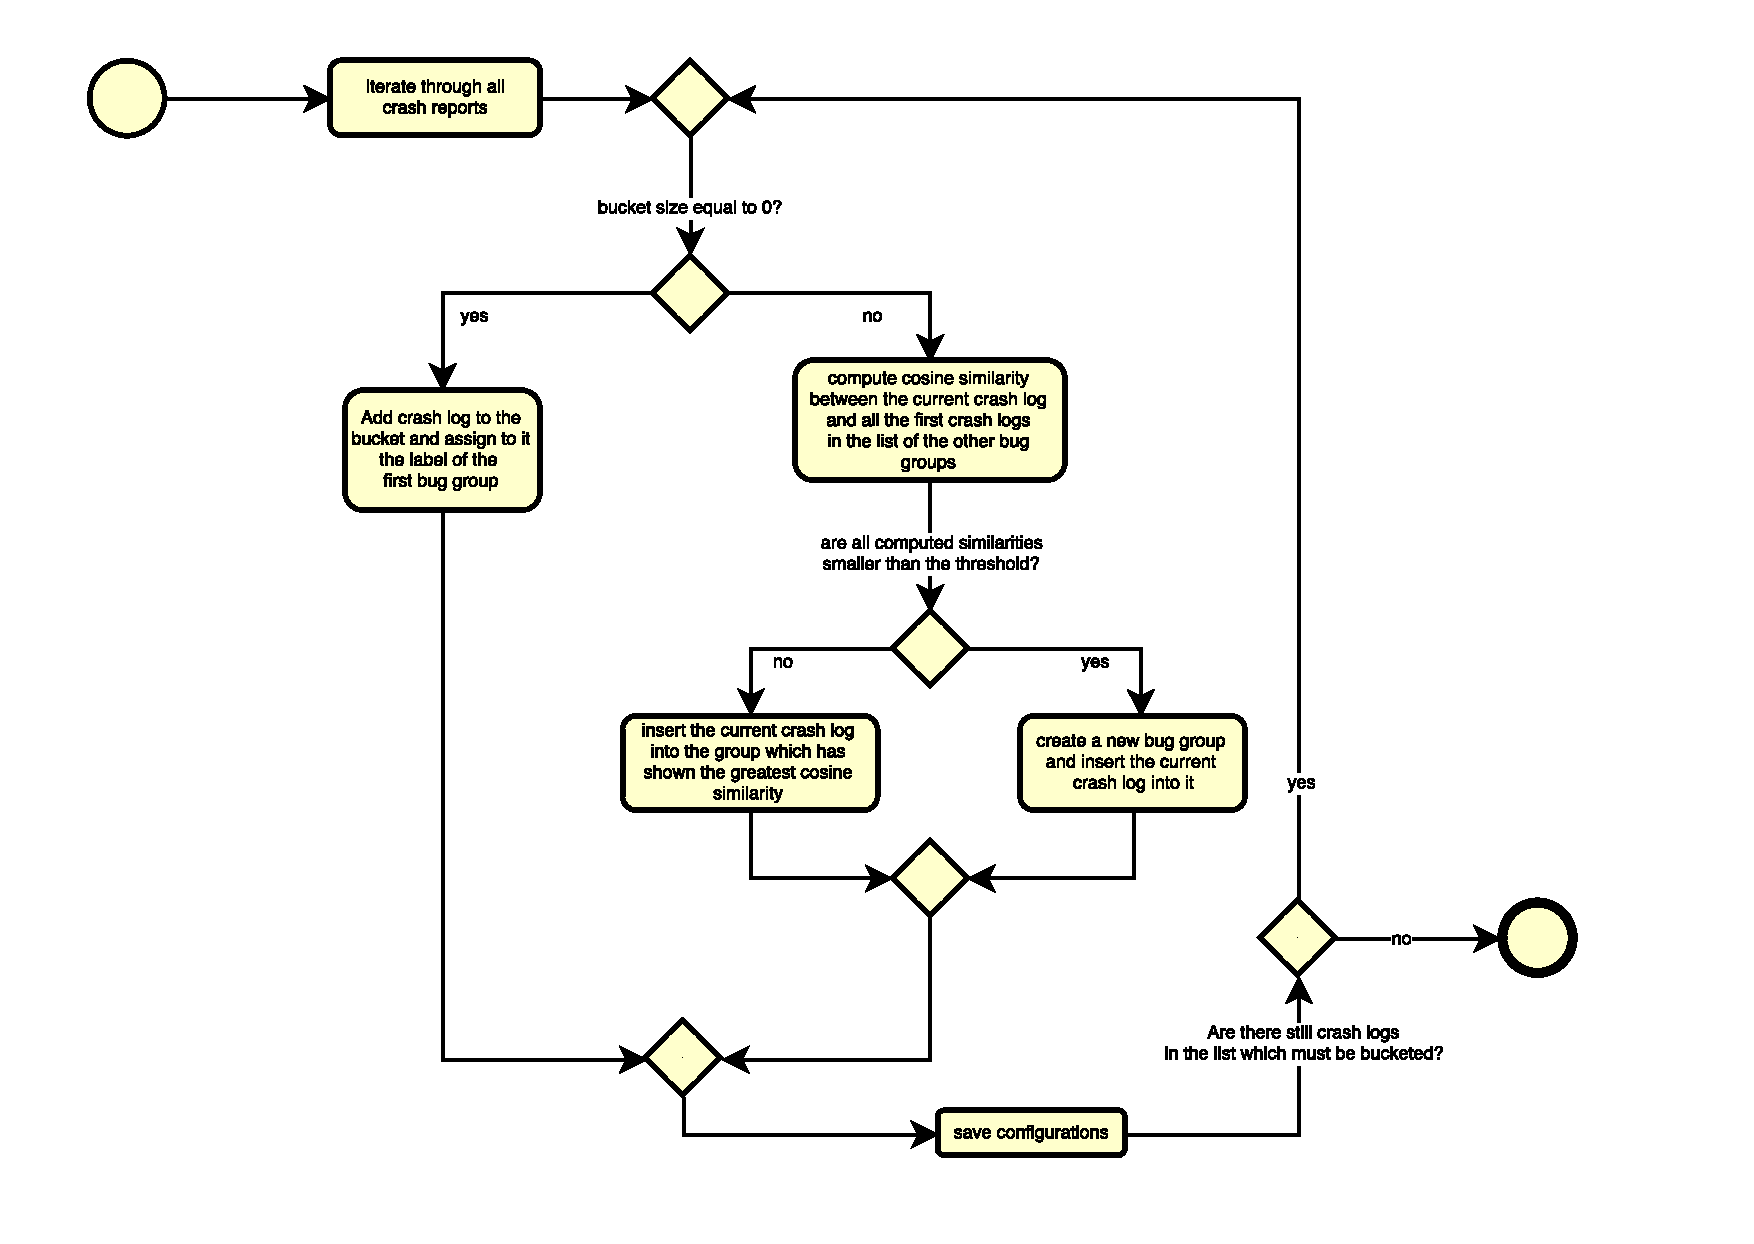
\includegraphics[width=\columnwidth]{diagrams/bucketingprocess.pdf} 
\caption{BPMN diagram describing the bucketing process}
\label{bucketing}
\end{figure}

%At the end of the bucketing process, \toolname\ saves the bucket and print it out. The clustering process is now completed. 
%conclusioni fare meglio

\section{Linking}
aaaaaaa

\section{How to start \toolname}
First of all, a set of parameters and directories have to inserted in the static \textit{Configuration Manager} file.
% qui inserire la command-line

\begin{figure}[htb]
\centering 
%	\vspace{-1.5mm} 
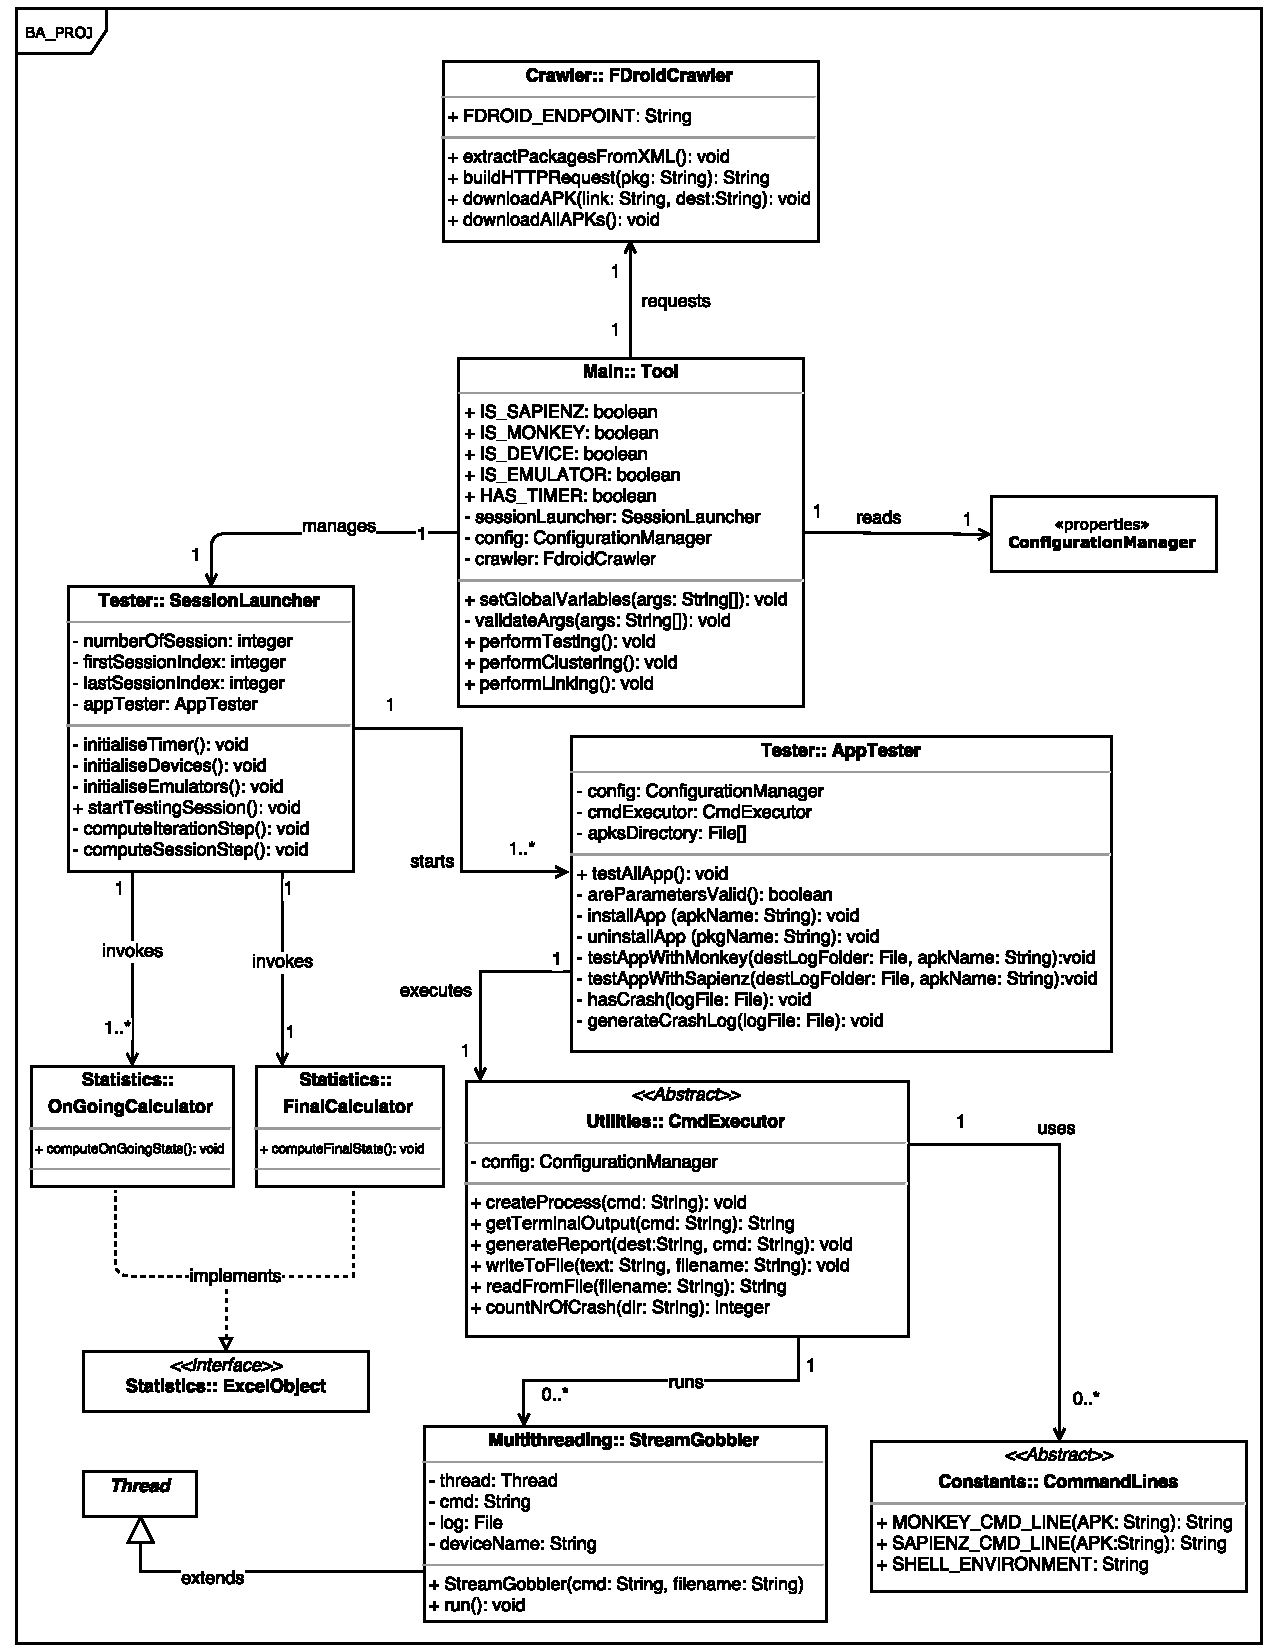
\includegraphics[width=\columnwidth]{diagrams/testing.pdf} 
\caption{Class Diagram of the testing part of the tool }
\label{testing}
\vspace{-3mm} 
\end{figure}


\begin{figure}[t]
\centering 
%	\vspace{-1.5mm} 
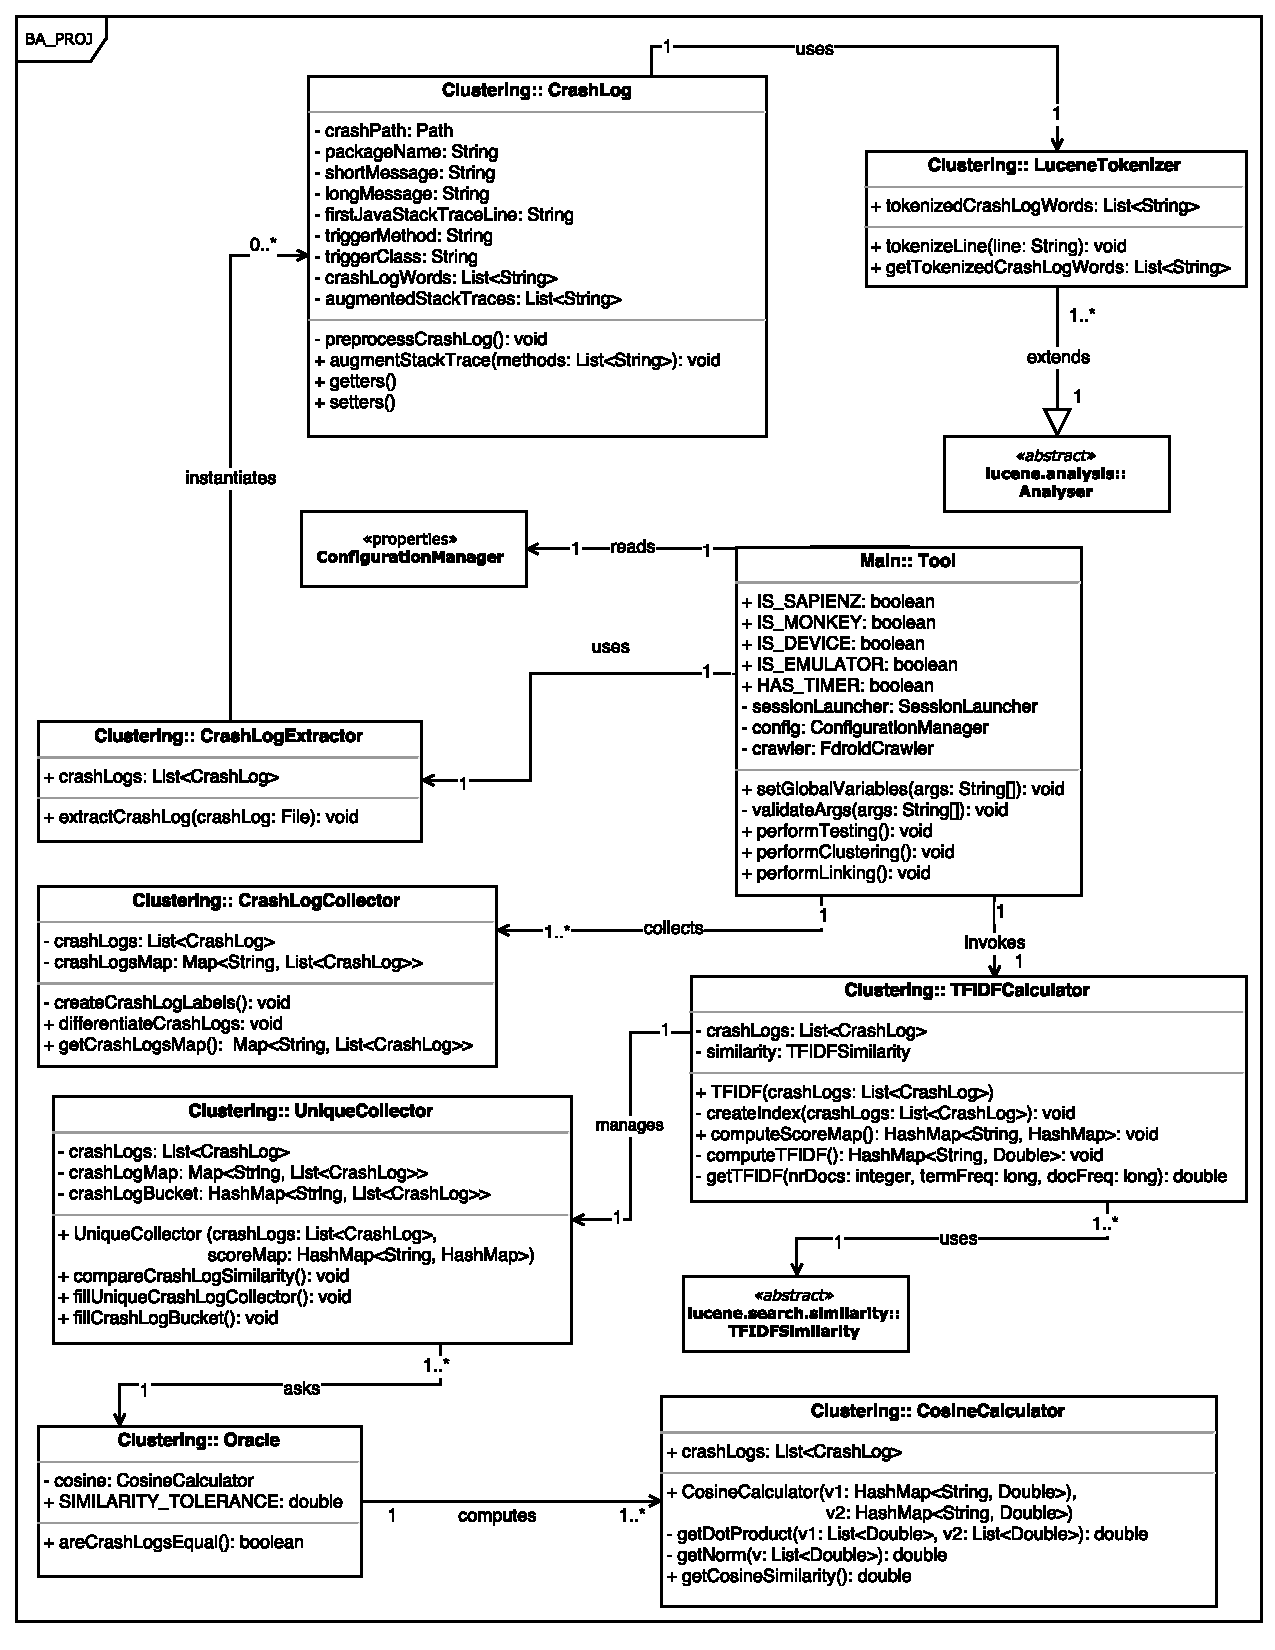
\includegraphics[width=\columnwidth]{diagrams/clustering.pdf} 
\caption{Class Diagram of the clustering part of the tool }
\label{clustering}
\vspace{-3mm} 
\end{figure}


\begin{figure}[t]
\centering 
%	\vspace{-1.5mm} 
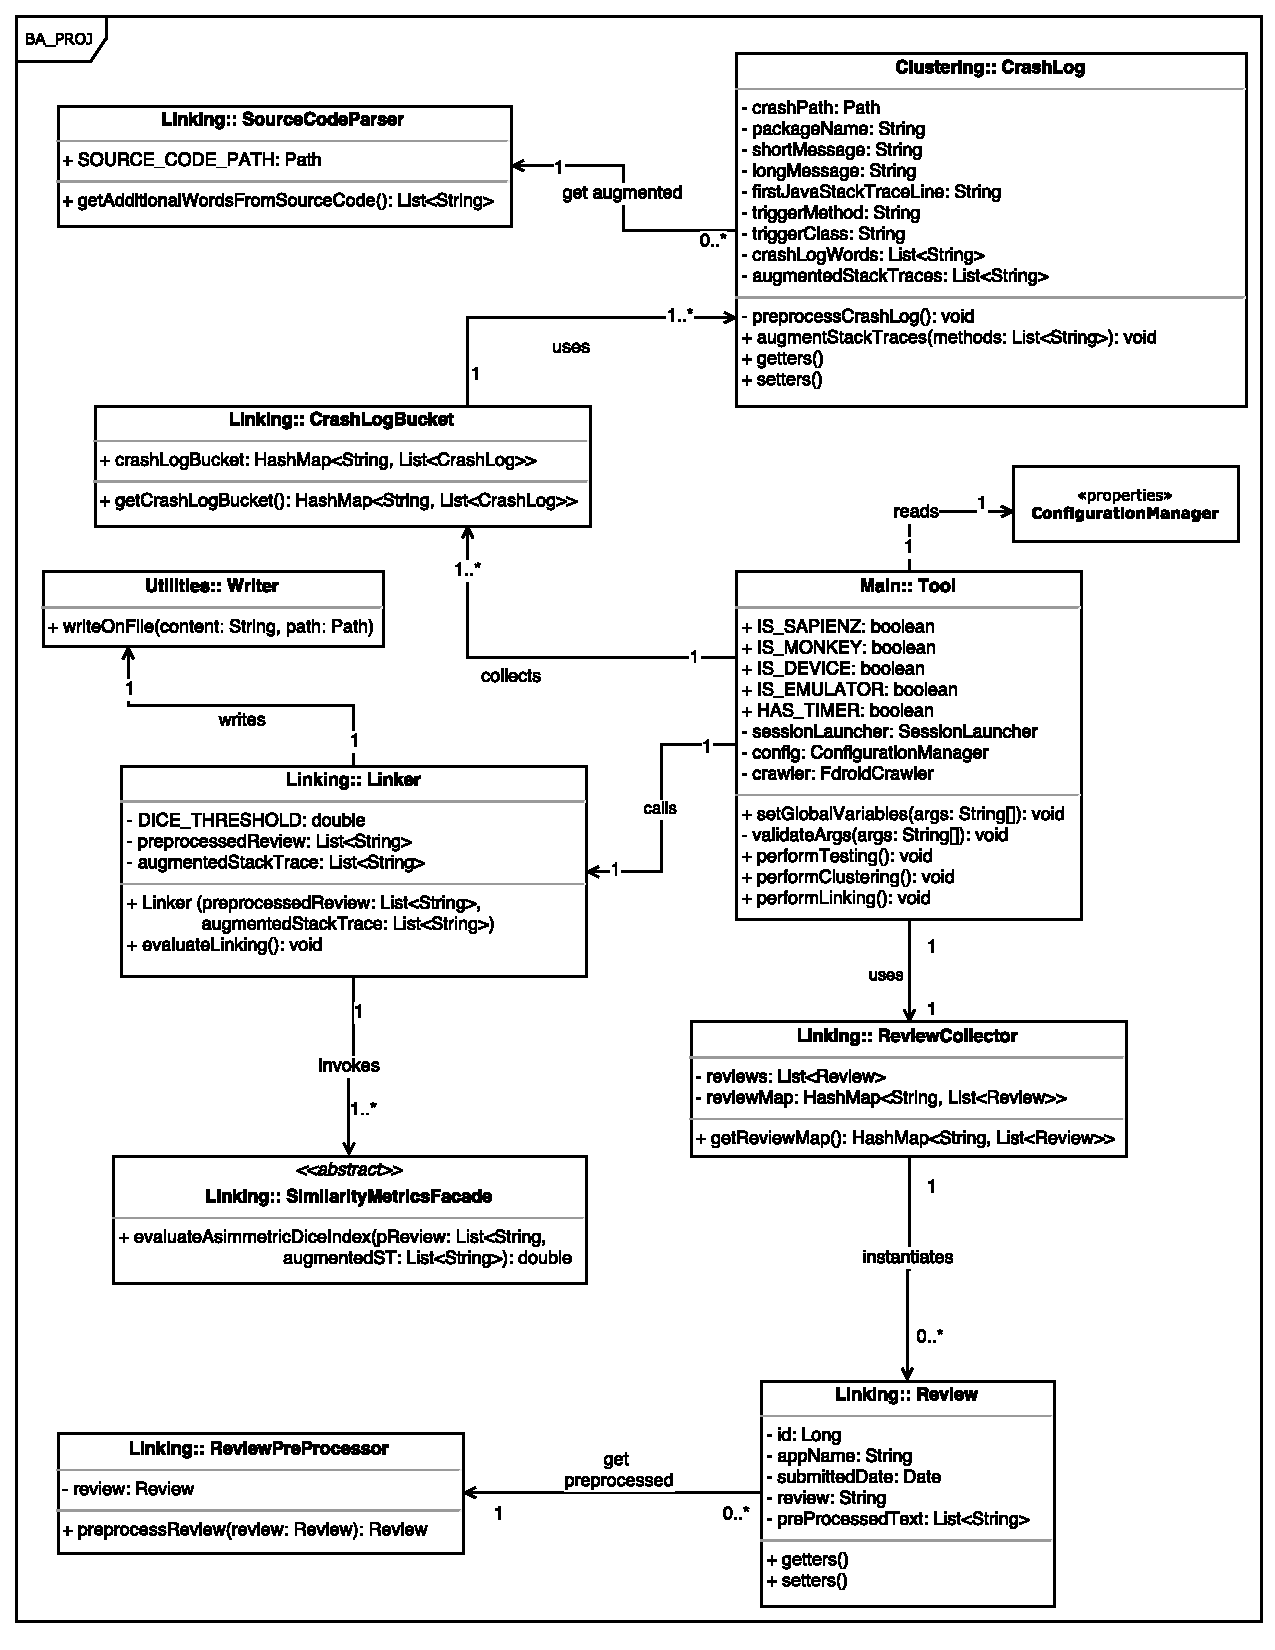
\includegraphics[width=\columnwidth]{diagrams/linking.pdf} 
\caption{Class Diagram of the linking part of the tool }
\label{linking}
\vspace{-3mm} 
\end{figure}